\documentclass[border=5pt]{standalone}
\usepackage{tikz}
\usetikzlibrary{shapes,arrows,positioning}

\begin{document}
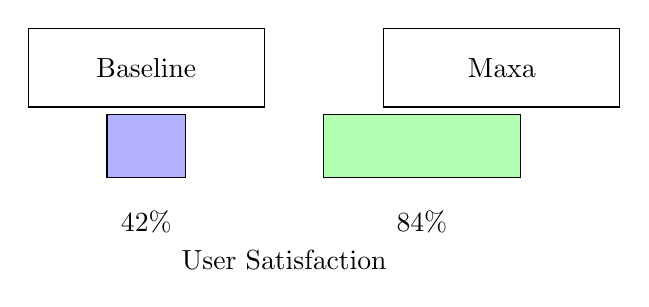
\begin{tikzpicture}[node distance=1.5cm, auto]
    % Nodes
    \node[draw, rectangle, minimum width=3cm, minimum height=1cm] (baseline) {Baseline};
    \node[draw, rectangle, minimum width=3cm, minimum height=1cm, right=of baseline] (maxa) {Maxa};
    
    % Bars
    \node[draw, fill=blue!30, minimum width=1cm, minimum height=0.8cm] at (0,-1) {};
    \node[draw, fill=green!30, minimum width=2.5cm, minimum height=0.8cm] at (3.5,-1) {};
    
    % Labels
    \node[below=0.2cm] at (0,-1.5) {42\%};
    \node[below=0.2cm] at (3.5,-1.5) {84\%};
    \node[below=0.7cm] at (1.75,-1.5) {User Satisfaction};
\end{tikzpicture}
\end{document}
